\documentclass[10pt,journal]{IEEEtran}
\IEEEoverridecommandlockouts
\usepackage[spanish,es-tabla]{babel}
\renewcommand{\baselinestretch}{1.5}     %interlineado
\usepackage[utf8]{inputenc} 
\usepackage[square,numbers]{natbib}
\bibliographystyle{abbrvnat}
\usepackage{float}                      % para usar [H]
\usepackage[table,xcdraw]{xcolor}
\usepackage{amsmath,amssymb,amsfonts}
\usepackage{graphicx}
\usepackage{textcomp}
\usepackage{xcolor}

\def\BibTeX{{\rm B\kern-.05em{\sc i\kern-.025em b}\kern-.08em
    T\kern-.1667em\lower.7ex\hbox{E}\kern-.125emX}}

%---------------------------------------------------
\begin{document}

\title{Usos de las Listas Enlazadas \\}
%--------------------------------------------
\author{\IEEEauthorblockN{Ciara Mendez Cruz}
\IEEEauthorblockA{\textit{} \\
\textit{Universidad Nacional de Trujillo} \\ 
\textit{Trujillo, Perú} \\
t022700920@unitru.edu.pe}}
\maketitle
%-------------------------------------------
\begin{abstract}
Las listas enlazadas son estructuras lineales y dinámicas de datos. La principal ventaja del dinamismo lo representa el hecho que adquieren posiciones de memoria a medida que se necesitan y se liberan cuando ya no se requieren. Es decir, se llegan a expandir o contraer, dependiendo de la aplicación. El dinamismo de estas estructuras soluciona el problema de decidir cuánto espacio se necesita a priori, por ejemplo, en una estructura de datos estática como el arreglo. Entre muchas de sus aplicaciones tenemos a los punteros y listas vinculadas en el análisis de circuitos de distribución de energía eléctrica, también un modelo de contacto combinado de semi-resorte y semi-borde en CDEM y su análisis en el deslizamiento de Jiweishan.
\end{abstract}

\begin{IEEEkeywords}
listas enlazadas, tecnologías, usos, dispositivos, aplicaciones.
\end{IEEEkeywords}

\section{\textbf{Introducción}}
Las listas enlazadas son un TDA (tipo de datos abstracto) que nos permite almacenar datos de una forma organizada,puesto que, es una estructura dinámica, por lo que no tenemos que saber 'a priori' los elementos que puede contener. Por ello, en este informe se presenta información respecto a las listas enlazadas, el cual está organizado de la siguiente manera: en primer lugar, se explican los conceptos teóricos de las listas enlazadas, luego se da énfasis en sus operadores básicos de una lista enlazada, finalmente se presenta seis de sus aplicaciones en el mundo, los cuales están presentes en los circuitos de energía eléctrica, en el deslizamiento de tierra, en el motor de búsqueda web, en su gestión a través de técnicas sin bloqueo, en aplicaciones de macrodatos basados en la nube y en bloques de construcción para aplicaciones colaborativos.
%------------------------------------------
\section{\textbf{Listas enlazadas}}
%\vspace{-22 mm}
\subsection{\textbf{Conceptos teóricos}}
%\vspace{-14 mm}
La lista enlazada es un TDA que nos permite almacenar datos de una forma organizada, al igual que los vectores pero, a diferencia de estos, esta estructura es dinámica, por lo que no tenemos que saber 'a priori' los elementos que puede contener.

En una lista enlazada, cada elemento apunta al siguiente excepto el último que no tiene sucesor y el valor del enlace es null. Por ello los elementos son registros que contienen el dato a almacenar y un enlace al siguiente elemento. Los elementos de una lista, suelen recibir también el nombre de nodos de la lista.
%-----------------------------------------------
\begin{figure}[H]
 \begin{center}
       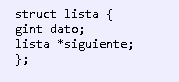
\includegraphics[width=5cm, height=3cm]{figuras/1.JPG}
      \caption{Estructura lista enlazada.}
      \label{f1} 
      \end{center}
\end{figure}
%------------------------------------------------
De la Figura~\ref{f1}, en la primera línea se representa el dato a almacenar. Puede ser de cualquier tipo; en este ejemplo se trata de una lista de enteros.\par
En la segunda línea se visualiza un puntero al siguiente elemento de la lista; con este puntero enlazamos con el sucesor, de forma que podamos construir la lista.

\subsubsection{\textbf{Operadores básicos de una lista enlazada}}
Para que esta estructura sea un TDA lista enlazada, debe tener unos operadores asociados que permitan la manipulación de los datos que contiene.\par

Los operadores básicos de una lista enlazada son:
%-------------------------------------
\begin{table}[H]
\centering
\caption{Operadores básicos de una lista enlazada.}
\label{tab1}
\begin{tabular}{|
>{\columncolor[HTML]{C0C0C0}}l l|}
\hline
\multicolumn{2}{|c|}{\cellcolor[HTML]{329A9D}{\color[HTML]{000000} \textbf{Operadores básicos}}} \\ \hline
\multicolumn{1}{|l|}{\cellcolor[HTML]{C0C0C0}{\color[HTML]{000000} \textbf{Insertar}}} & {\color[HTML]{000000} \begin{tabular}[c]{@{}l@{}}Inserta un nodo con dato x en la lista,\\ pudiendo realizar esta inserción al\\ principio, al final o en orden.\end{tabular}} \\ \hline
\multicolumn{1}{|l|}{\cellcolor[HTML]{C0C0C0}{\color[HTML]{000000} \textbf{Eliminar}}} & {\color[HTML]{000000} \begin{tabular}[c]{@{}l@{}}Elimina un nodo de la lista, puede\\ ser según la posición o por el dato.\end{tabular}} \\ \hline
\multicolumn{1}{|l|}{\cellcolor[HTML]{C0C0C0}{\color[HTML]{000000} \textbf{Buscar}}} & {\color[HTML]{000000} Busca un elemento en la lista.} \\ \hline
\multicolumn{1}{|l|}{\cellcolor[HTML]{C0C0C0}{\color[HTML]{000000} \textbf{Localizar}}} & {\color[HTML]{000000} Obtiene la posición del nodo en la lista.} \\ \hline
\multicolumn{1}{|l|}{\cellcolor[HTML]{C0C0C0}{\color[HTML]{000000} \textbf{Vaciar}}} & {\color[HTML]{000000} Borrar todos los elementos de la lista.} \\ \hline
\end{tabular}
\end{table}
%---------------------------------------------------------------------------
\section{\textbf{Aplicaciones de la lista enlazada}}
No es necesario que la lista esté presente de forma contigua en la memoria. El nodo puede residir en cualquier lugar de la memoria y vincularse para hacer una lista. Esto logra una utilización optimizada del espacio.
El tamaño de la lista está limitado al tamaño de la memoria y no es necesario declararlo por adelantado.
El nodo vacío no puede estar presente en la lista vinculada.
Podemos almacenar valores de tipos u objetos primitivos en la lista enlazada individualmente.
Por ello, a continuación se presenta seis de sus aplicaciones:


%----------------------------------    
\subsection{\textbf{Punteros y listas vinculadas en el análisis de circuitos de distribución de energía eléctrica}}
Los programas de análisis de circuitos de distribución de energía eléctrica deben administrar de manera eficiente una gran cantidad de datos de sistemas y equipos. Los ingenieros de servicios públicos ahora desean utilizar paquetes de software integrados con varias funciones que funcionan de manera eficiente y comparten datos. En este articulo \citep{energia} se describe el uso de estructuras de datos almacenadas en listas enlazadas y procesadas mediante punteros. Los punteros y las listas vinculadas compactan el almacenamiento de datos y reducen los tiempos de ejecución del algoritmo. Varios algoritmos pueden compartir funciones de gestión de datos y gráficos, lo que reduce el costo de mejorar y mantener el código. El enfoque de este articulo se aplico a un paquete de software que integra gráficos, gestión de datos, análisis y algoritmos de diseño.
%----------------------------------    
\subsection{\textbf{Un modelo de contacto combinado de semi-resorte y semi-borde en CDEM y su aplicación al análisis del deslizamiento de tierra de Jiweishan}}
De acuerdo a \citep{semi}, el método de elementos discretos basado en el continuo (CDEM) es un método numérico explícito utilizado para la simulación de falla progresiva del cuerpo geológico. \par Para mejorar la eficiencia de la detección de contacto y simplificar los pasos de cálculo de las fuerzas de contacto, se introducen en el cálculo el semirresorte y el semifilo.
\begin{itemize}
    
    \item \textbf{El semirresorte} \par
    El semirresorte se deriva del vértice del bloque y se forma al sangrar el vértice del bloque en cada cara (24 semirresorte para un elemento hexaédrico). El proceso de formación del semi-borde es el mismo que el del semi-resorte (24 semi-bordes para un elemento hexaédrico). A partir de los semi-resortes y semi-bordes, se presenta un nuevo tipo de modelo de contacto combinado. 
\end{itemize}
De acuerdo con este modelo, seis tipos de contacto podrían reducirse a dos, es decir, el contacto de la cara del objetivo con semirresorte y el contacto con el borde del objetivo con semiborde. Mediante el modelo combinado, la fuerza de contacto podría calcularse directamente (la información del tipo de contacto no es necesaria), y el juicio de falla podría ejecutarse de una manera sencilla (cada semi-resorte y semi-borde posee sus áreas características).
%-----------------------------------------------
\begin{figure}[H]
 \begin{center}
       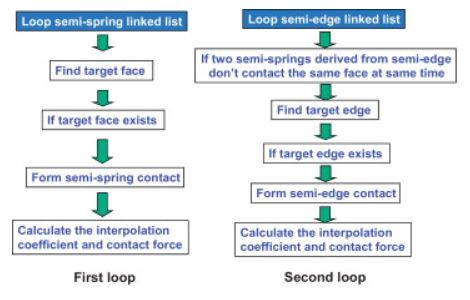
\includegraphics[width=8cm, height=4cm]{figuras/2.JPG}
      \caption{Dos listas enlazadas en el modelo de contacto combinado.}
      \label{f2} 
      \end{center}
\end{figure}
%------------------------------------------------
El algoritmo presentado en este articulo se programo con éxito en el programa C ++. En este existen dos listas vinculadas principales en el programa, lista vinculada semi-resorte y lista vinculada semi-borde. Para buscar contactos, los bucles de estas listas enlazadas se ejecutan respectivamente, y los detalles de cada bucle se muestran en la Figura~\ref{f2} .Se presentan algunos casos numéricos simples para mostrar la validez y precisión de este modelo. Finalmente, el modo de falla, distancia de deslizamiento y crítica. El ángulo de fricción del deslizamiento de tierra de Jiweishan se estudia con el modelo combinado.
%----------------------------------    
\subsection{\textbf{La aplicación del algoritmo de reglas de asociación en el motor de búsqueda web}}
Con el objetivo de abordar el problema de minería predominantemente preocupado sobre la construcción de la búsqueda de conceptos en el área actual del motor de búsqueda web (Figura~\ref{f3}), especialmente aplicando el modelo de espacio vectorial VSM a la minería de búsqueda web basada en las reglas de asociación, \citep{lu}, en su articulo proporciona un algoritmo de minería altamente eficiente EARS.
%-----------------------------------------------
\begin{figure}[H]
 \begin{center}
       
\includegraphics[width=8cm, height=4cm]{figuras/3.JPG}
      \caption{Ejemplos de principales motores de búsqueda.}
      \label{f3} 
      \end{center}
\end{figure}
%------------------------------------------------
El algoritmo EARS implementa la poda de reglas de asociación basada en VSM mediante la construcción de una biblioteca de asociación y similitud informática. El EARS almacena los conjuntos de elementos frecuentes a través de listas enlazadas multidimensionales y utiliza la relación de recurrencia entre los conjuntos de elementos frecuentes para obtener de manera eficaz las reglas de asociación.Además se Verifico la función extendida de recuperar y consultar en la Web y los resultados de estos experimentos indicaron que el método es efectivo y factible.
%----------------------------------    
\subsection{\textbf{Gestión de listas enlazadas largas mediante técnicas sin bloqueo}}
%-----------------------------------------------
\begin{figure}[H]
 \begin{center}
       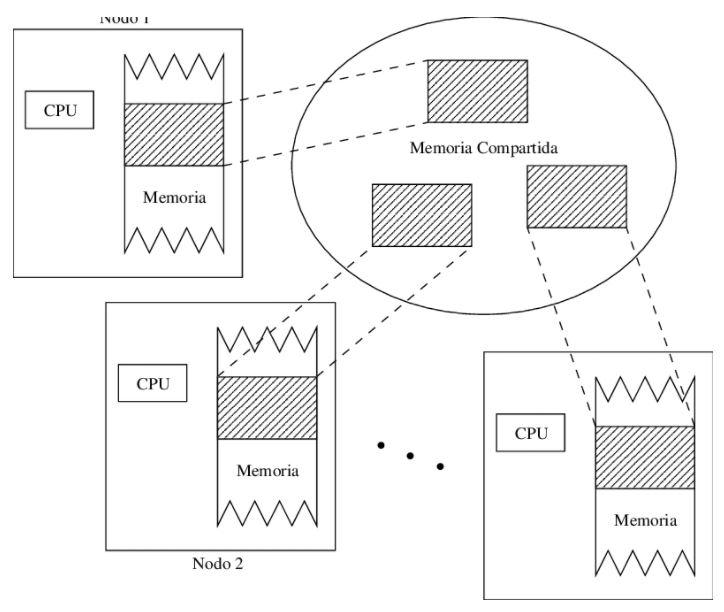
\includegraphics[width=8cm, height=4cm]{figuras/4.JPG}
      \caption{Sistema de Memoria Compartida Distribuida.}
      \label{f4} 
      \end{center}
\end{figure}
%------------------------------------------------
Al escribir programas paralelos para máquinas de memoria compartida como muestra la Figura~\ref{f4}, es común utilizar estructuras de datos compartidas (listas enlazadas, colas, árboles, etc. ).\par El control de simultaneidad para tales estructuras de datos puede implementarse usando sincronización de bloqueo o sin bloqueo / sin bloqueo. El bloqueo de la sincronización es popular porque es familiar y también susceptible de análisis de rendimiento en el peor de los casos (importante para ciertas aplicaciones en tiempo real). Desafortunadamente, también adolece de algunas características indeseables. Estos incluyen la posibilidad de un punto muerto, concurrencia limitada debido a que los procesos están bloqueados y ciertas anomalías de programación. Las técnicas de no bloqueo, aunque menos frecuentes, no sufren estos problemas y pueden ser adecuadas para muchos problemas de programación paralela.\par
A pesar del mayor interés en las técnicas de no bloqueo, incluso las estructuras de datos simples, como las listas enlazadas individualmente, a menudo tienen limitaciones molestas.  \citep{faro} en su articulo presenta una nueva implementación de listas enlazadas sin bloqueo que supera algunos problemas comunes con las implementaciones existentes.\par Además de ofrecer una mayor simultaneidad general, la técnica presentada también aumenta significativamente el rendimiento de las listas enlazadas largas. \citep{faro} también proporciona algoritmos para el recorrido, la inserción y la eliminación de listas, y mostramos su exactitud. También analiza los resultados de un estudio de simulación que compara el desempeño de su implementación con dos técnicas existentes bajo diferentes condiciones de carga y patrones de acceso y para varias longitudes de lista.
%----------------------------------    
\subsection{\textbf{Predicción del rendimiento de aplicaciones de macrodatos basadas en la nube}}
La heterogeneidad y la irregularidad de los datos son características clave de las aplicaciones de big data que a menudo abruman las infraestructuras de software y hardware existentes.\par En tal contexto, la flexibilidad y elasticidad que brinda el paradigma de la computación en la nube sobre un enfoque natural para adaptar de manera rentable los recursos asignados a las necesidades actuales de la aplicación. \par Sin embargo, las mismas características imponen desafíos adicionales para predecir el rendimiento de las aplicaciones de big data basadas en la nube, un paso central en la gestión y planificación adecuadas. En su articulo, \citep{arda} explora dos enfoques de modelado para la predicción del rendimiento de aplicaciones de big data basadas en la nube. Evaluan un modelo analítico basado en colas y un nuevo simulador ad-hoc rápido en varios escenarios basados en diferentes aplicaciones y configuraciones de infraestructura. Nuestros resultados muestran que nuestros enfoques pueden predecir los tiempos promedio de ejecución de aplicaciones con un 26\% de error relativo en el peor de los casos y alrededor del 12\% en promedio. Además, su simulador proporciona estimaciones de rendimiento 70 veces más rápido que las herramientas de simulación de última generación.

Mediante el uso de una lista doblemente enlazada que almacena la información relevante sobre las tareas pertenecientes a las etapas en el estado CAN.START, es posible determinar cuál se puede ejecutar sin realizar una búsqueda completa en el conjunto completo de tareas en el DAG. En este sentido, el enfoque proporcionado por el motor de dagSim es original y más eficiente con respecto a otros mecanismos de programación implementados en herramientas de propósito general como JMT o GreatSPN.

%-----------------------------------------------
\begin{figure}[H]
 \begin{center}
       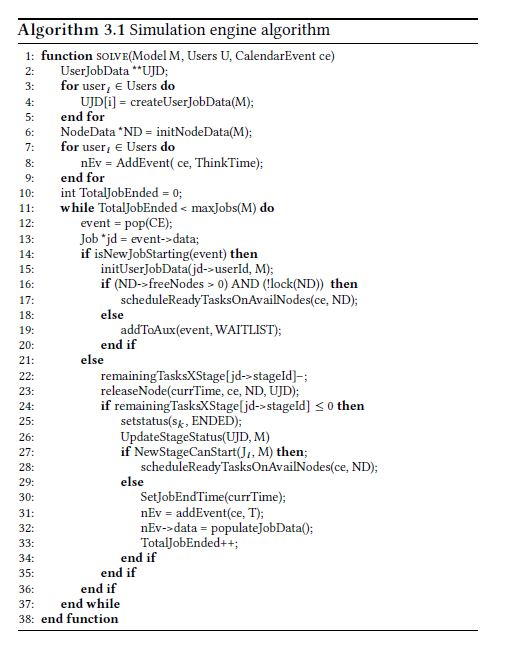
\includegraphics[width=8cm, height=9cm]{figuras/5.JPG}
      \caption{El algoritmo para simular la ejecución de un trabajo de acuerdo con el DAG dado.}
      \label{f5} 
      \end{center}
\end{figure}
%------------------------------------------------

El algoritmo (Figura~\ref{f5}) resume el procedimiento para simular la ejecución de un trabajo de acuerdo con el DAG dado. Inicialmente (líneas 2-5), para cada uno de los usuarios de NUsers que acceden al sistema, se llena una lista doblemente enlazada llamada UJD con un conjunto de información, en particular:
\begin{enumerate}
    \item El número de etapas listas para comenzar.
    \item Las tareas restantes que deben completarse para cada etapa.
    \item El estado de cada etapa.
    \item La hora de inicio y finalización de cada etapa.
    \item Un puntero a una lista de trabajos listos para comenzar.
\end{enumerate}

%----------------------------------------------
\subsection{\textbf{Tipos de datos abstractos replicados: bloques de construcción para aplicaciones colaborativas}}
Para las aplicaciones distribuidas que requieren colaboración, se desea una interactividad receptiva y transparente. Aunque tal interactividad se puede lograr con una replicación optimista, mantener la consistencia de la réplica es difícil. Para respaldar implementaciones eficientes de aplicaciones colaborativas, por lo que, \citep{ro} en su documento amplía algunos tipos de datos abstractos representativos (ADT), como matrices, tablas hash (Figura~\ref{f6}) y matrices que pueden crecer (o listas vinculadas), en tipos de datos abstractos replicados (RADT). \par En RADT, un ADT compartido se replica y modifica con operaciones optimistas. Operación conmutatividady la transitividad de precedencia son dos principios que permiten a los RADT mantener la coherencia a pesar de las diferentes órdenes de ejecución. Especialmente, las matrices de crecimiento replicadas (RGA) admiten operaciones de inserción / eliminación / actualización. Con respecto a los enfoques anteriores para la inserción y eliminación optimistas, los RGA muestran una mejora significativa en el rendimiento, la escalabilidad y la confiabilidad.
%-----------------------------------------------
\begin{figure}[H]
 \begin{center}
       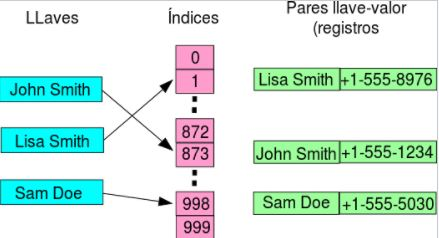
\includegraphics[width=8cm, height=4cm]{figuras/6.JPG}
      \caption{Ejemplo de Tabla Hash.}
      \label{f6} 
      \end{center}
\end{figure}
%------------------------------------------------
\section{\textbf{Conclusiones}}
Este informe presentó información relevante acerca de las principales aplicaciones de las listas enlazadas, se ha explicado los conceptos teóricos relacionados con estas, además de permitir conocer sobre su presencia en los circuitos de energía eléctrica, en el deslizamiento de tierra, en el motor de búsqueda web, en su gestión a través de técnicas sin bloqueo, en aplicaciones de macrodatos basados en la nube y en bloques de construcción para aplicaciones colaborativos.
%-------------------------------------------------------
\medskip
\bibliography{refer}
\end{document}
